\documentclass[a4paper]{article}

\usepackage{cruz_article}

\renewcommand{\arraystretch}{2}

\title{User Interface Evaluation of the CP's Website\\ (Proposal)}
\author[1]{Luís  Cruz}
\affil[1]{MAP-i\\ Joint Doctoral Programme in Computer Science}
\date{January 4, 2014}

\begin{document}
\maketitle

%----------------------------%
%          ABSTRACT          %
%----------------------------%
\begin{abstract}
This document proposes an usability evaluation for the website of the company \emph{CP -- Comboios de Portugal}.
One analytical method and one empirical method are going to be applied in this evaluation: \emph{Heuristic Evaluation} and the \emph{Usability Test}, respectively, both described in this document.
  
Through the Heuristic evaluation it was possible to find X issues in the user interface.
As a result of the usability test a report complying with the CIF standards, an usability test plan, and a usability post-test questionnaire were produced. The usability test assessed the efficiency, efficacy and satisfaction measures of the system.
\todo{talk about }

\end{abstract}

\section{Introduction}

This project aims to evaluate the user interface of CP.pt\footnote{Available at: \url{http://www.cp.pt}} --- the official website of \emph{CP - Comboios de Portugal, E.P.E}.

CP is a public portuguese company responsible for rendering national and international passenger rail services. In the year 2012, CP had 4690 employees, transported 122 million passengers and almost 8713 thousand metric tons~\citep{CP2012aa}. They provide 3 main kinds of rail transportation services: \emph{urban} in the cities of Oporto and Lisbon; \emph{National} with regional services and the fast lines of \emph{Alfa Pendular} and \emph{Intercidades}; and \emph{International}.

Through the website, CP's customers can check the timetables, buy tickets, get information about the available lines and special offers and read some news related with CP services. In order to buy tickets, the website provides the \emph{netTicket} service, which requires the customers to have an account in their \emph{myCP} service and it is only available for the long distance trains \emph{Intercidades} and \emph{Alfa Pendular}.

According to the website the graphical interface was optimally designed for windows with $800\times 600$ pixels of resolution. A view of the website is depicted in the figure~\ref{fig:cp_home}, using a window with the same resolution. 

\begin{figure}[h] 
	\centering
	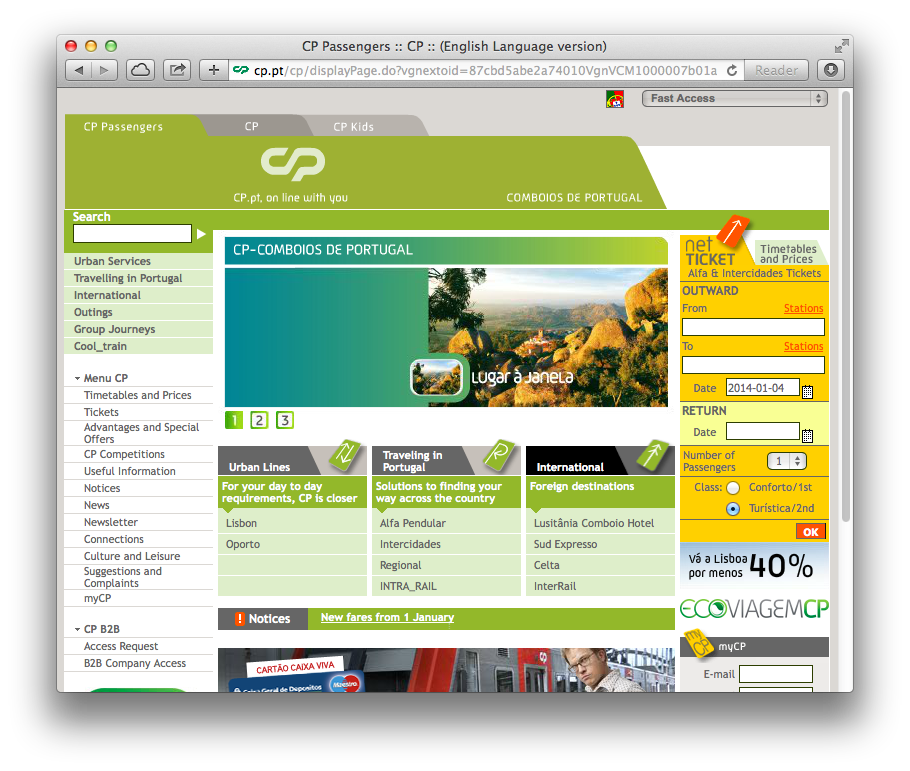
\includegraphics[width=\textwidth]{figures/cp_home}
 	\caption{View of the main page of CP.pt website in a window with resolution $800\times 600$ pixels, using the internet browser Safari Version 7.0.1.}\label{fig:cp_home}
\end{figure}

\section{Users and Context}
\label{sec:users_context}

CP customers vary according to the service provided. Many college students, workers and pensioners use the regional and urban services for small and medium distances. Long distance services are more used by college students that are away from home, tourists, and executive workers. Unfortunately, no official document stating the segmentation of the CP.pt website's users was found.

It is noticeable that CP services have a lot more passengers during school time, which means that students are an important segment of CP's customers. Besides, most of the students have good experience with the WEB, so the CP.pt website is expected to be a great tool to them. Therefore, this usability evaluation will focus in the segment of college students, which might be portuguese citizens as well as foreigners that study or want to study in Portugal and are able to speak English.

Many scenarios can apply for the use of the website by students. Some times they leave the classes earlier and need a way of quickly check if there are other alternative trains that can take them home earlier. Also sometimes there is no direct train to their destination, so they have to catch another in the the middle of the traveling. Another scenario is when the weekend is over and the student has to buy his/her ticket from home to his/her university city. Buying it from the website is more convenient since the student can avoid wasting time in the ticket lines and can grant a seat for his/her trip. Therefore, the following two contexts are considered the most important in terms of usability:

\begin{itemize}
  \item Check the timetable to find any suitable train for the trip and the respective prices.
  \item Buy a ticket for long distance trains with reserved seats.
\end{itemize}

\section{Usability Evaluation Methodology}

The evaluation will be taken using two paradigms: \emph{Analytical} and \emph{Empirical}.

\emph{Analytical} methods do not need to involve users --- they are based on inspection methods. Some well known analytical methods are the \emph{Heuristic Evaluation} (HE) proposed by \citet{nielsen1990heuristic}, the \emph{Cognitive Walkthrough} \citep{wharton1994cognitive} and its variant \emph{Streamlined Cognitive Walkthrough} \citep{spencer2000streamlined}.

\emph{Empirical} methods involve the user in the evaluation process through Usability tests, involving \emph{observation} and \emph{query} techniques, through \emph{controlled experiments}, in a more scientific approach, or even \emph{questionnaires}, \emph{focus groups}, etc. 

In this evaluation, the used analytical method will be the \emph{Heuristical Evaluation} and the empirical method will be the \emph{Usability Test}. These methods are described in the next sections.



%----------------------------------------------------------------------------------------
%	Heuristic Evaluation
%----------------------------------------------------------------------------------------
\section{Heuristic Evaluation}

The elected analytical method for this evaluation was the \emph{Heuristic Evaluation}, because it is cheap, intuitive, easy to motivate people to do it and provides that useful results can be obtained~\citep{nielsen1990heuristic}.

\subsection{Methodology}
This method proceeds by having a small set of evaluators judging the system according to some general principles of interaction design, \emph{usability heuristics}. It has been shown that a number of evaluators between 3 and 5 provides good results and that there is no point in having more than 10 evaluators \citep{nielsen1990heuristic}. \citet{nielsen1995ten} proposed the 10 most important usability heuristics for User Interface Design:

\begin{itemize}
	\item Visibility of system status

	\item Match between system and the real world

	\item User control and freedom

	\item Consistency and standards

	\item Error prevention

	\item Recognition rather than recall

	\item Flexibility and efficiency of use

	\item Aesthetic and minimalist design

	\item Help users recognize, diagnose, and recover from errors

	\item Help and documentation.
\end{itemize}

Heuristic evaluation was originally developed for evaluators who had some knowledge in usability but who were not necessarily usability experts~\citep{nielsen1990heuristic}, however, it has been showed that the method is also very effective for expert evaluators~\citep{nielsen1992finding}.

In order to group the findings of this heuristic evaluation, the severity ranking proposed by \citet{nielsen1995rating} with a scale from 0 to 4:

\begin{enumerate}[start=0, label={\theenumi{} -}]
\item I don't agree that this is a usability problem at all;
\item Cosmetic problem only: need not be fixed unless extra time is available on project;
\item Minor usability problem: fixing this should be given low priority;
\item Major usability problem: important to fix, so should be given high priority;
\item Usability catastrophe: imperative to fix this before product can be released.
\end{enumerate}

In this evaluation, two experienced evaluators were asked to focus on the interface elements related with the following top-level user stories:
\begin{itemize}
  \item As an unregistered user I want to check time tables and prices for traveling from a given train station to another one.
  \item As an unregistered user I want to buy a ticket for the fast train services \textit{Alfa Pendular} and \textit{Intercidades} (it may include a registration process).
\end{itemize}

\subsection{Results}

After completing the heuristic evaluation \todo{number of problems} 11 problems were found. They were sorted in table~\ref{tab:heuristic_results} according to the severity rating.
\begin{table}[h]
\begin{center}
  \footnotesize
\begin{tabular}{c | p{8cm} | c | p{4.5cm}}
  \hline
	\# & Problem & \parbox[c]{1cm}{Severity Rating} & Violated Heuristic(s)  \\
	\hline
	
		1  &  The ``Timetable and Prices" form is very similar with the form for buying tickets. Non expert users might not notice the difference.    & \cellcolor{red!25} 3 & Error prevention.  \\
		
		2 &  There is an auto complete feature in the ``Timetable and Prices'' and netTicket forms, which whenever the user misspells a letter of the station name, the system may complete with another station's name, and the user has to hit the backspace button one more time than usual. & \cellcolor{red!25} 3 & Error prevention; Help users recognize, diagnose, and recover from errors.\\
	
  3   & The seat selection is made in a uncommon way. One has to first click on the previous seat and then on the desired seat.  & \cellcolor{red!25} 3 &  Consistency and standards.  \\
  
		4  & The services of trains are defined as acronyms which are not used by the users (eg., IC means Intercidades)  &\cellcolor{orange!20} 2  &  Consistency and standards; Match between system and the real world.  \\
	

	5  &  When an unregistered user wants to buy a ticket after choosing a specific train, the system asks him/her to register but after finishing the registration, he/she has to search again for the same train.    & \cellcolor{orange!20} 2 &  Recognition rather than recall. \\

6 &  In order to check the price in the timetable it is necessary to click in a link which when clicked replaces itself into the respective price, but only for one train at a time. & \cellcolor{orange!20} 2 & Flexibility and efficiency of use.\\


7 &  When searching for a traveling ticket to buy, the user selects whether is traveling in first or second class in the beginning of the search. It is defined as second class by default and might not be perceptible. Through the next steps the user cannot change it. & \cellcolor{orange!20} 2 & User control and freedom.\\

8 & In the buying process there is no back button, besides the one provided by the browser that is not recommended by the system since he presents an alert warning that the user is about to leave the page. & \cellcolor{orange!20}2 & User control and freedom.\\

9  &  In the timetable results, there is a clickable down arrow that does not do anything  & \cellcolor{yellow!10} 1 &  Aesthetic and minimalist design; Consistency and standards.  \\

	10  &  There is a Time input field when in the form ``Timetables and Prices'', which might be unnecessary and provides no useful filtering in the results.  & \cellcolor{yellow!10} 1 &  Aesthetic and minimalist design.  \\
	
		11 &  In the timetable results there is a number identifying the row that does not provide any useful information & \cellcolor{yellow!10} 1 & Aesthetic and minimalist design.\\
	
\hline
\end{tabular}
\end{center}
\caption{Problems found in the Heuristic Evaluation.}
\label{tab:heuristic_results}
\end{table}


%----------------------------------------------------------------------------------------
%	USABILITY TEST
%----------------------------------------------------------------------------------------
\section{Usability Test}

The usability test was carefully reported using the Common Industry Format (CIF)~\citep{iusr2006cif} in a document entitled \emph{Usability Test Report} which is provided in the appendix~\ref{sec:usabilityTestReport}. This section briefly describes the usability test, but for further details please refer to the usability test report.

Furthermore, in the scope of this test, an \emph{Usability Test Plan}, and a \emph{Post-Test Questionnaire} were designed, being all available in the appendix of the usability test report (see appendix~\ref{sec:usabilityTestReport}). Additionally, all material and data can be downloaded in this assignment project's website\footnote{This assignment is published in a website available at~\url{http://paginas.fe.up.pt/~luiscruz/cp_usability/}}.

\paragraph{Participants} Two individuals were invited to participate. They were college students complying ages between 21 and 26 years, and they usually have to travel in order to get to their universities. All participants had a moderate level of experience using WEB applications.

\begin{samepage}
\paragraph{Methodology} The users were invited to perform some tasks regarding some of the most used features in the website:

\begin{enumerate}
  \item Select the English Version of the application.
  \item Find the schedule for a trip from Braga to Aveiro.
  \item Find a cheap trip from Braga to Aveiro.
  \item Buy a ticket from Braga to Porto.
\end{enumerate}
\end{samepage}

As suggested in~\citep{mitchell2007step} it is beneficial to get the participant's opinion during the test session.
The usability test combined both \emph{observation} and \textit{query}.

The participants were asked to use the think aloud behavior (TA), describing every step they made during the tasks.
The moderator was directly observing the participant while taking some notes using the \emph{Data Logging Form}, and after the completion of each task, users were interviewed in a casual way, trying to answer some questions clearly stated in the \emph{Usability Test Plan} document.
In addition, the screen and audio were also recorded for indirect observation.
 
All this setup intended to evaluate the system in terms of \emph{effectiveness}, \emph{efficiency}, and \emph{user satisfaction}:
 
 \begin{itemize}
   \item Effectiveness
   \begin{itemize}
     \item Completion Rate
     \item Unassisted completion rate
     \item Number of assistances
     \item Number of steps made differently
     \item Back Button hits
     \item Errors
   \end{itemize}
   \item Efficiency
   \begin{itemize}
     \item Task time
     \item Completion rate efficiency
   \end{itemize}
   \item User satisfaction
   \begin{itemize}
     \item SUS scale
   \end{itemize}
 \end{itemize}
 \todo{fill variables}
 
 After the completion of each task, users were interviewed in an informal way, trying to answer some questions clearly stated in the \emph{Usability Test Plan} document. Moreover, after the whole test, participants gave some feedback through the \emph{Post-Test Questionnaire}.
 
 
 \paragraph{Main Results}
All users were able to successfully complete the given tasks, and the assisted completion rate was 75\%.

The first task, selecting the english version, was very simple and users took just 8 seconds to complete. This task proved that the feature is well implemented, and was important to make the participant comfortable with the test environment. The task 4, buying a ticket, was more complex and took longer for the users to complete, with an average of 6 minutes and 27 seconds. The efficiency was also measured through the completion rate efficiency, resulting in a mean of $38\%/min$.

The time results suggest an interesting fact in the times for task 2 and task 3. The complexity of these tasks is very similar and the steps to complete are identical. However, task 2 took in average 2 minutes and 38 seconds, while task 3 reduced this time to 1 minute and 9 seconds. This can be an indicator that the system might be well suited for second time visitors.

Some times the user was confused and made wrong steps, but easily recognized and hit the back button. This inefficiency was reported with an average of 2.5 hits per user during the whole test.

The SUS questionnaire scored 60 points. In~\citep{sauro2011measuring}, the average SUS for 500 systems is 68, which means that this website has a satisfaction level considered below average. According to a SUS qualitative classification proposed in~\citep{bangor2009determining}, the overall satisfaction perceived from users is \textbf{good}.

\paragraph{Observed issues and users's feedback}
One very important contribution of the interviews and the post-test questionnaire was to get the most from the user's opinion. This procedure successfully provided some spots in the features that need improvement. 

Users are satisfied with the graphical appearance of the website. However, they stated that is too much information in the view.

An important issue was the fact of the ``Timetable and Prices'' form is not visible but is very similar to the \emph{netTicket} form which is visible. Users frequently made the mistake of using the wrong form. Another component users didn't like was the table results. They felt the need of a more readable table that provided some filtering, at least for price range and line service.

Another difficulty faced by first time users, was the feature of selecting a seat for the ticket. The user interaction was intuitive and users had negative remarks about that.

\paragraph{Pilot Test}

Although some statistical analysis was performed, the sample of users is not representative due to its small size (two individuals). This means that, although some important considerations were taken and which might help to improve the usability of the website, the measures reported cannot be considered as valid. 
The state of this study can be seen as the starting point for a rigorous usability test with more participants.  \todo{usability test size of sample}

However, this experiment allowed to make a pilot test: some aspects of the test were iteratively improved, and some other might need some changes in future work.

Some of the changes made were regarding the interview for each task. The interview guidelines tried to answer the same generic questions in different tasks, which did not provide any extra information. This was improved from the first to the second participant.
Another small fix that had to be made was to increase the size of the fields in the post-test questionnaire, since they were too small.

In the first attempts for the screen and audio recording, each task was being recorded separately. This was leading to an interruption of the flow of the test, because the moderator had to start and stop the recording each time. Thus, it was decided to record the session in a single take.

One of the main difficulties was the think aloud technique. It is hard to make a participant feel really comfortable to explain every single step. Also, it depends on the profile of the participant, some participants might be more quiet than others. Another aspect to improve is the fact of users sometimes want to prove they have good skills, and do not want to make mistakes, which makes harder to reproduce the usual behavior of the user.

Regarding the Data Logging Form, some measures did not provide useful measures and could be removed in future experiments in order to simplify the observation process. This is the case of \emph{time start}, \emph{time end}, and \emph{number of negative remarks}. Regarding \emph{negative remarks}, it is important to write down this feedback in the notes field, but the number of remarks was not very useful in this case.

Another change that could be made is related with the interviews made after each task. They are very useful, but some of the questions made were not

% ---------------~o~--------------- %



% ------------ RESULTS ------------ %
\section{Conclusions and Future Work}

This document reported the usability evaluation of CP.pt website. The \emph{Heuristic Evaluation} was very effective, it allowed to find 11\todo{FIXME} usability problems, from which 3 were considered to be high priority fixes. Besides, it was very cheap and easy to prepare. Before proceeding to the usability test, this issued should have been fixed.

The usability test provided was carefully prepared and two college students participated in the experiment.
An usability test plan with some guidelines, a post-test questionnaire, a SUS questionnaire, and a data logging form were developed to get a very detailed information about the usability.
The results suggest that website is very effective, since all users were able to correctly complete all the tasks, with an assisted completeness rate was of 75\%. 

\todo{talk about satisfaction, interview and questionnaire}

Although the size of the sample was to small, the experiments with these 2 participants served as a pilot test, allowing to improve the test procedure and tools. As future work, the designed usability test should be conducted with a more representative sample. For better results, the problems spotted with the Heuristic Evaluation should be fixed before proceeding with the usability test.
% ---------------~o~--------------- %

\appendix


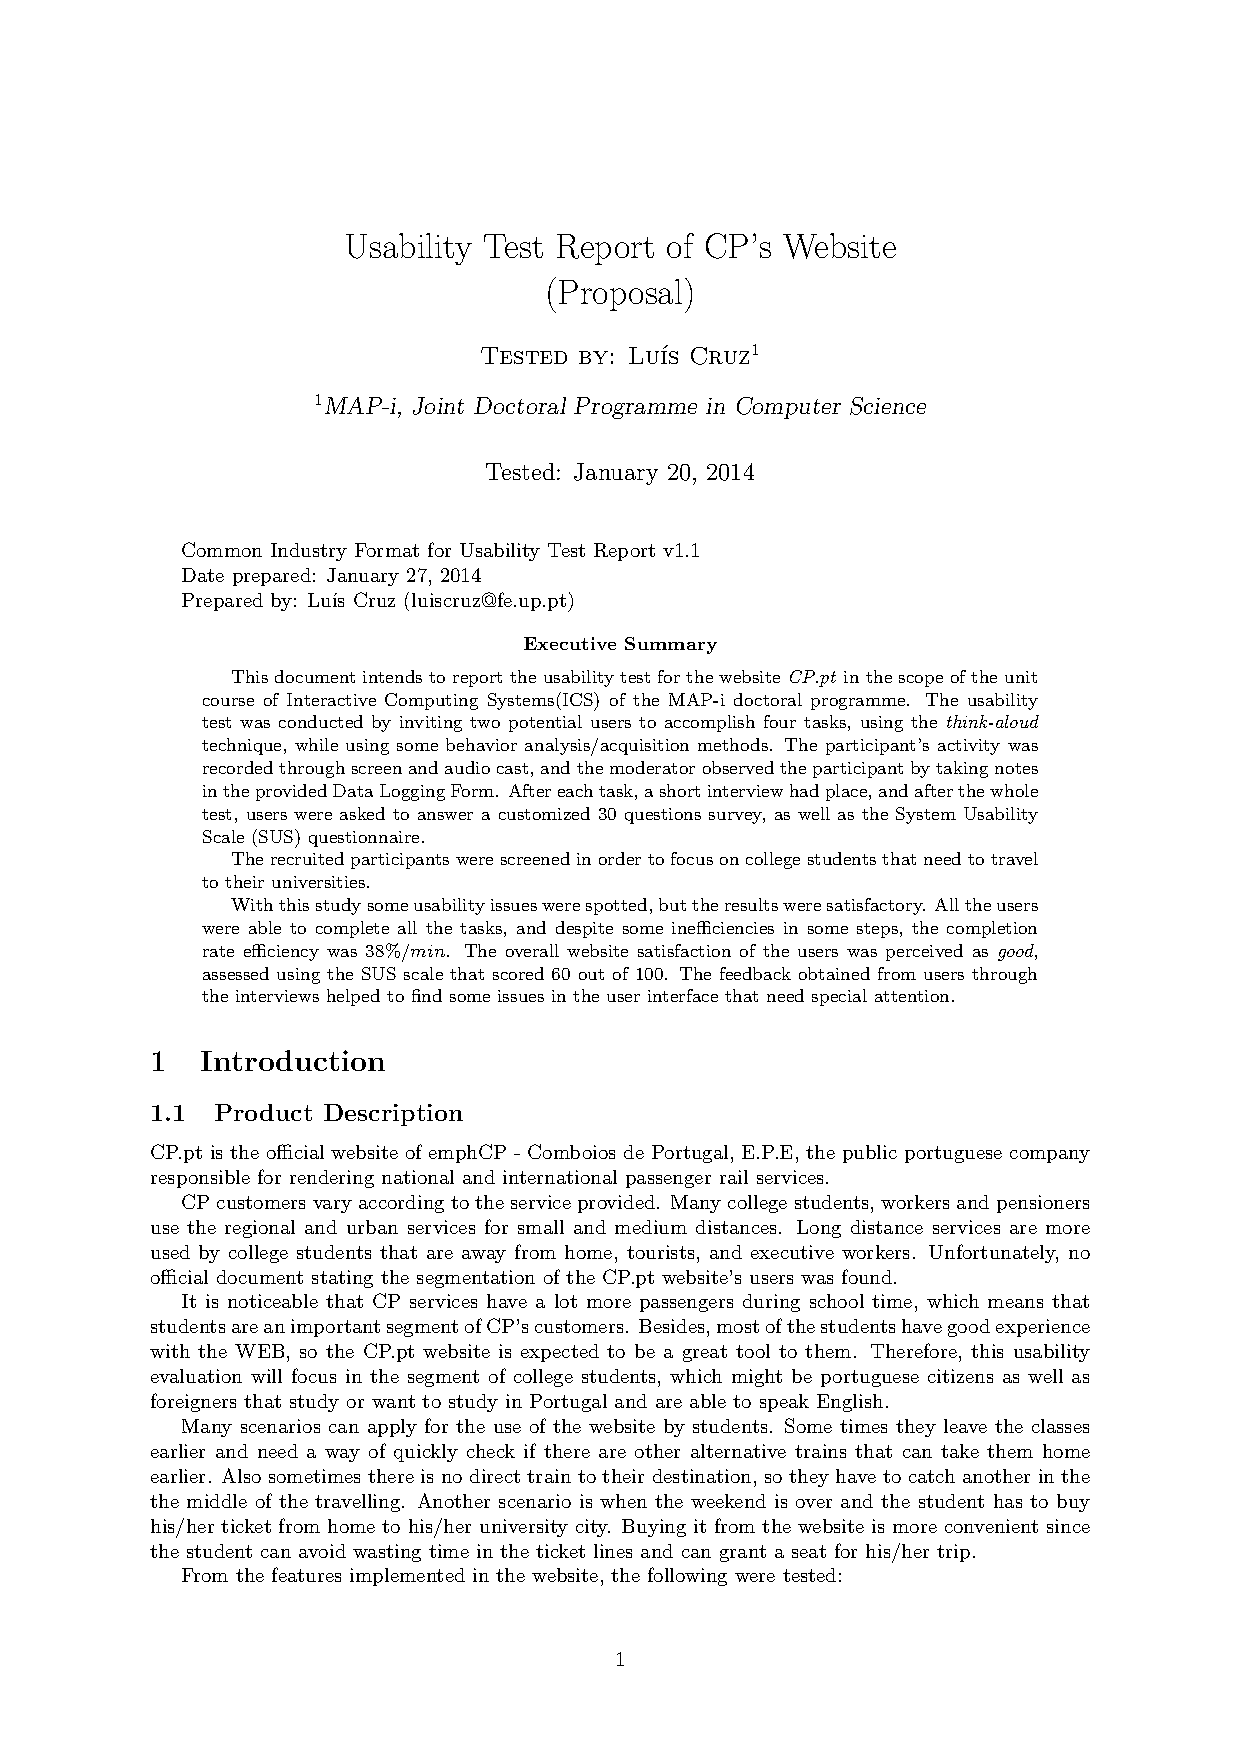
\includepdf[pagecommand=\section{Usability Test Report}\label{sec:usabilityTestReport}\thispagestyle{plain}{The original document is available at \url{http://paginas.fe.up.pt/~luiscruz/cp_usability/}}, pages=1, frame=true, scale=0.75, offset=0 -25]{../usabilityTestReport/master.pdf}

\includepdf[pagecommand=\thispagestyle{plain}, pages=2-, nup=2x2, frame=true, scale=0.8]{../usabilityTestReport/master.pdf}

% ---------------~o~--------------- %


%----------------------------------------------------------------------------------------
%	BIBLIOGRAPHY
%----------------------------------------------------------------------------------------

\bibliographystyle{apalike}
\bibliography{../bibliography}

%----------------------------------------------------------------------------------------

\end{document}